\chapter{Evaluation}
\label{chap:evaluation}

In this chapter the methods for performing the experimental evaluation of this
work are presented and the results are discussed. The evaluation was split into
two parts. The first part consists of a custom microbenchmark that uses the
\lib library directly. The second part consists of known programs making use of
the new forwarding mechanism transparently via the modified C library.

\section{System and Configuration}

All measurements presented in this chapter were taken on a Raspberry Pi 3 Model
B which uses a Broadcom BCM2837 system on a chip (SoC) with a 1.2 GHz 64-bit
quad-core ARM Cortex-A53. The board's CPU contains 32KB of L1 cache (split into
16KB i-cache and 16KB d-cache), 512KB of L2 cache and the SoC is linked to a
1GB LPDDR2 memory module. Of this memory, 450MB was allocated to the
para-virtualized \llinux instance.

Memsc was implemented in the \llinux kernel version 5.6.0 which for the
purposes of this evaluation ran on top of the L4Re version 20.07. Due to
incomplete support of Fiasco's decoupling mechanism for the ARM 64-bit
architecture, the 32-bit version of all the aforementioned software was used.
The CPU also ran in its 32-bit mode of operation.

By default the Raspberry Pi performs dynamic CPU frequency scaling. This means
that the CPU frequency is automatically adjusted on the fly depending on the
system workload in order to conserve power and reduce the amount of heat
generated by the chip. Since this behavior can affect measurements, it was
completely disabled. Instead, the system was setup to always operate at the
maximum frequency of 1.2GHz. Disabling the automatic CPU frequency scaling was
achieved by setting the \emph{force\_turbo} option on Raspberry's
\emph{config.txt} configuration file.

Buildroot \cite{buildroot} was used for generating a small root filesystem
containing only the necessary system binaries and libraries, benchmarking code,
and the modified C library based on the uclibc-ng version 1.0.32. No periodic
jobs or unnecessary services ran during benchmarking. The root file system of
type rootfs\footnote{rootfs is a special instance of tmpfs, an in-memory file
system} was loaded in memory and was not backed by a block device.

For measuring the passage of time, the ARM architecture provides a generic
timer and a set of counters. Among these, there is a 64-bit per-core virtual
timer whose value can be obtained by reading the contents of the CNTVCT counter
register. This counter is incremented with a constant frequency determined by
the value stored in the CNTFRQ register (19.2MHz by default on the Raspberry Pi
3). Fiasco is configured to allow user-level code to access these registers.
The custom benchmark programs used the virtual timer in order to measure
execution time.

To avoid measurement noise and wasted cycles caused by process migration to
different cores, the benchmark processes were pinned on a single CPU core
during their execution. This was achieved by setting the process affinity using
the \emph{taskset} utility. The first physical CPU was used in the case of
native Linux and the first vCPU in the case of \llinux.  The L4 vCPU threads
are by default non-migratable, therefore they always execute on the same
physical core as well.

For the \llinux experiments, two vCPUs were made available to \llinux always
executing on the 3rd and 4th physical core correspondingly. When decoupling was
used, the benchmark application was decoupled to the 1st physical core. That
is, in the decoupling test cases the benchmark ran as a decoupled thread on the
1st core, forwarding its system calls to the 3rd core (hosting the 1st vCPU) of
the Raspberry. In the Memsc case, the 4th core (hosting the 2nd vCPU) was used
for running the scanner thread. This setup is identical to the one depicted in
Figure \ref{fig:architecture} with the only difference being that the 2 vCPUs
were swapped.

All values reported in this evaluation represent the average of 5 separate
runs. The standard deviations of these runs were calculated and found to be
low; less than 5\% of the mean value for all experiments and less than 1\% of
the mean value for most file system tests.

\section{Custom Microbenchmarks Using Memsclib}

For the first part of this experimental evaluation a simple microbenchmark that
executes a number of getppid system calls in a loop and then exits was used.
This custom program explicitly makes use of the \memsc interfaces by linking
against \lib directly, making it possible to use the asynchronous execution
capabilities of \memsc as well. The getppid system call was chosen because it
requires a minimal amount of work in the kernel allowing the focus to be on the
round trip times of the forwarding mechanism (whenever cross-processor
forwarding was required).

First the execution time using blocking system calls was measured, followed by
experiments using batched execution of system calls. Finally, the system
throughput with multiple decoupled threads running in parallel was computed.

\subsection{Synchronous System Calls}

For the first experiment, the benchmark was run for an increasing number of
system calls. The program had to block and wait after issuing each system call
until it was processed by the kernel and the result was ready. Performance was
compared among native Linux, \llinux without decoupling, \llinux with
decoupling, and \memsc-patched \llinux with decoupling.

Table \ref{tab:block_single} and Figure \ref{fig:block_single} present the
results of these tests. The ``dec" column indicates whether or not the
decoupling mechanism was used in the corresponding experiment. As expected,
\llinux being virtualized is always slower than native Linux. We also confirm
that when the decoupling mechanism is used, there is a very significant
performance overhead due to the cross-processor forwarding of system calls.

\newcommand\Aa{4}
\newcommand\Ab{7}
\newcommand\Ac{39}
\newcommand\Ad{307}
\newcommand\Ae{2938}
\newcommand\Af{25618}

\newcommand\Ba{10}
\newcommand\Bb{41}
\newcommand\Bc{348}
\newcommand\Bd{3423}
\newcommand\Be{34260}
\newcommand\Bf{342381}

\newcommand\Ca{36}
\newcommand\Cb{278}
\newcommand\Cc{2701}
\newcommand\Cd{26949}
\newcommand\Ce{269664}
\newcommand\Cf{2705248}

\newcommand\Da{27}
\newcommand\Db{143}
\newcommand\Dc{1205}
\newcommand\Dd{11702}
\newcommand\De{116112}
\newcommand\Df{1163886}

\begin{table}[h]
\centering
  \begin{tabular}{ |p{2.9cm}|p{0.5cm}|p{0.8cm}|p{1cm}|p{1.2cm}|p{1.3cm}|p{1.4cm}|p{1.6cm}| }
 \hline
    \multicolumn{2}{|c|}{Blocking syscalls} & \multicolumn{6}{c|}{Number of system calls} \\
 \hline
    OS kernel & dec & 1 & 10 & 100 & \num{1000} & \num{10000} & \num{100000} \\
 \hline
 \hline
    Linux & no & \num{\Aa} & \num{\Ab} & \num{\Ac} & \num{\Ad} & \num{\Ae} & \num{\Af} \\
 \hline
    \llinux & no & \num{\Ba} & \num{\Bb} & \num{\Bc} & \num{\Bd} & \num{\Be} & \num{\Bf} \\
 \hline
    \llinux & yes & \num{\Ca} & \num{\Cb} & \num{\Cc} & \num{\Cd} & \num{\Ce} & \num{\Cf} \\
 \hline
    \llinux-\memsc & yes & \num{\Da} & \num{\Db} & \num{\Dc} & \num{\Dd} & \num{\De} & \num{\Df} \\
 \hline
\end{tabular}
  \caption{Times (in microseconds) for completing a fixed number of blocking
  system calls per kernel and thread execution mode}
\label{tab:block_single}
\end{table}

\begin{figure}[h]
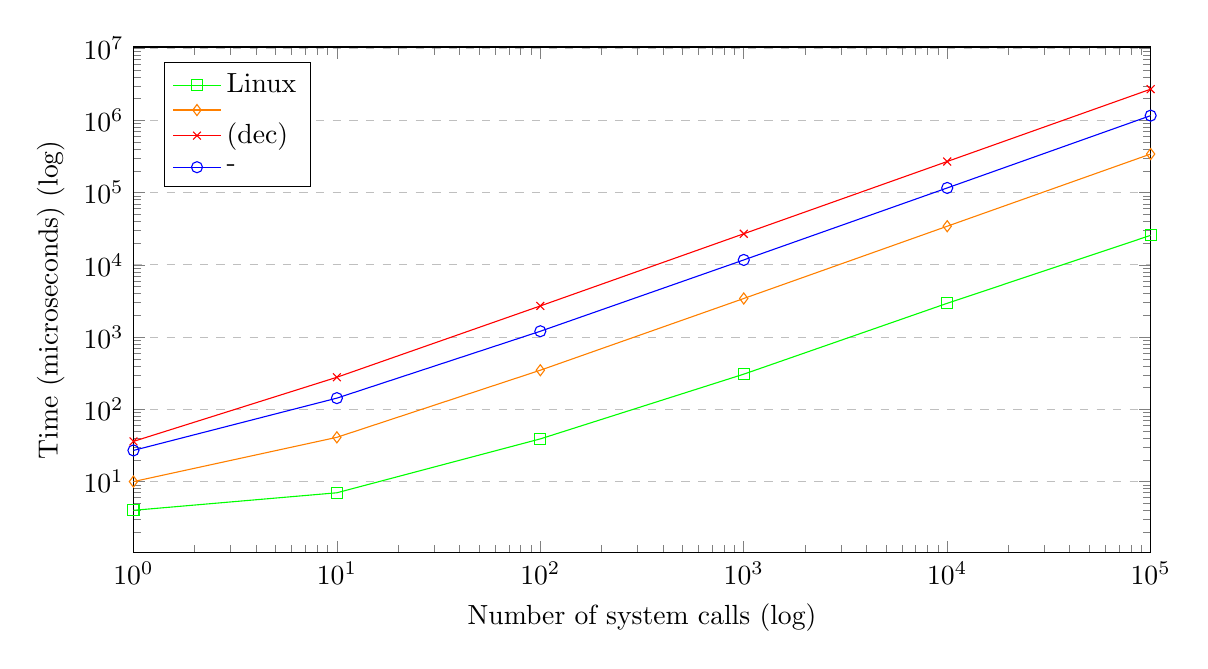
\begin{tikzpicture}
\begin{loglogaxis}[
    height=8cm,
    width=14.5cm,
    xlabel={Number of system calls (log)},
    ylabel={Time (microseconds) (log)},
    xmin=1, xmax=100000,
    xtick={1, 10,100,1000,10000,100000},
    ymajorgrids=true,
    grid style=dashed,
    legend pos=north west,
    legend cell align={left},
    legend entries = {Linux, \llinux, \llinux (dec), \llinux-\memsc}
]

\addplot[color=green, mark=square] coordinates {
  (1,\Aa)(10,\Ab)(100,\Ac)(1000,\Ad)(10000,\Ae)(100000,\Af)
};

\addplot[color=orange, mark=diamond] coordinates {
  (1,\Ba)(10,\Bb)(100,\Bc)(1000,\Bd)(10000,\Be)(100000,\Bf)
};

\addplot[color=red, mark=x] coordinates {
  (1,\Ca)(10,\Cb)(100,\Cc)(1000,\Cd)(10000,\Ce)(100000,\Cf)
};

\addplot[color=blue, mark=o] coordinates {
  (1,\Da)(10,\Db)(100,\Dc)(1000,\Dd)(10000,\De)(100000,\Df)
};

\end{loglogaxis}
\end{tikzpicture}
\caption{Comparison of blocking system calls performance among different
  configurations}
\label{fig:block_single}
\end{figure}

\newcommand{\Ea}{\the\numexpr(\Ca-\Da)*100/\Da\relax}
\newcommand{\Eb}{\the\numexpr(\Cb-\Db)*100/\Db\relax}
\newcommand{\Ec}{\the\numexpr(\Cc-\Dc)*100/\Dc\relax}
\newcommand{\Ed}{\the\numexpr(\Cd-\Dd)*100/\Dd\relax}
\newcommand{\Ee}{\the\numexpr(\Ce-\De)*100/\De\relax}
\newcommand{\Ef}{\the\numexpr(\Cf-\Df)*100/\Df\relax}

\begin{figure}[h!]
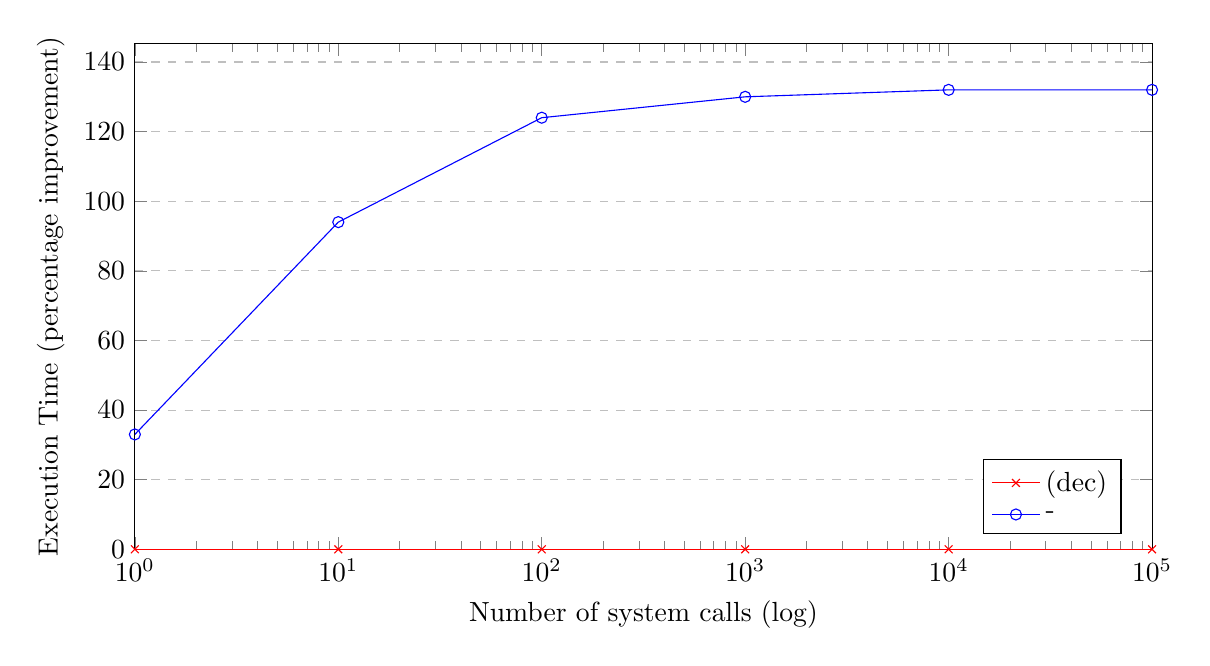
\begin{tikzpicture}
\begin{semilogxaxis}[
    height=8cm,
    width=14.5cm,
    xlabel={Number of system calls (log)},
    ylabel={Execution Time (percentage improvement)},
    xmin=1, xmax=100000,
    ymin=0,
    xtick={1, 10,100,1000,10000,100000},
    ymajorgrids=true,
    grid style=dashed,
    legend pos=south east,
    legend cell align={left},
    legend entries = {\llinux (dec), \llinux-\memsc}
]

\addplot[color=red, mark=x] coordinates {
  (1,0)(10,0)(100,0)(1000,0)(10000,0)(100000,0)
};

\addplot[color=blue, mark=o] coordinates {
  (1,\Ea)(10,\Eb)(100,\Ec)(1000,\Ed)(10000,\Ee)(100000,\Ef)
};

\end{semilogxaxis}
\end{tikzpicture}
\caption{Execution time percentage improvement of \llinux-\memsc versus
  standard \llinux when using blocking system calls}
\label{fig:block_single_per}
\end{figure}

What we are mostly interested in seeing is whether or not directly forwarding
system calls using shared memory is faster than forwarding them via
cross-processor IPC. We indeed observe that \memsc-patched \llinux performs
significantly better than standard \llinux with decoupling for any number of
system calls. In fact, for more than 10 system calls the execution is more than
twice as fast.

Figure \ref{fig:block_single_per} shows the execution time percentage
improvement\footnote{ Calculating percentage improvement for elapsed time where
smaller is better can be confusing. The formula used for calculating the
percentage is (old-new)/new*100\%. In this case a percentage improvement of
100\% means that the benchmark program ran twice as fast. } of \memsc-enabled
\llinux over standard \llinux. What we can see in this diagram is that for more
than 100 system calls there is a solid performance improvement of more than
120\% which goes up to 133\% for larger amounts of system calls.

\subsection{Asynchronous System Calls and Batching}

The previous section discussed the execution times for issuing blocking system
calls. This section focuses on asynchronous system calls and the batched
execution mode that the \memsc mechanism enables. In order to evaluate the
batching capabilities of \memsc, the getppid benchmark was run with 100,000
iterations and was repeated for different batch sizes.

At this point, it is worth reminding the reader that when using \memsc the
system calls are processed by the kernel as soon as possible after being posted
to the \sysp. Furthermore, the system call entries are posted to memory
individually by the \emph{memsc\_add} library call, instead of been posted
all together when a \emph{memsc\_wait\_all} call is made. That means that by
the moment the user program calls the \emph{memsc\_wait\_all} function, some
or all of the system calls posted might have already been completed.

The term batching is used a bit loosely here. It is about allowing the
user-space to make progress and not have to block after each and every system
call it issues. With the term ``batch size" we refer to the number of system
call entries that have been posted between two subsequent
\emph{memsc\_wait\_all} calls.  However when exactly the kernel will pick up
these entries for execution depends entirely on scheduling activity. The
\emph{memsc\_wait\_all} call serves as a barrier that doesn't allow the program
to proceed until all posted system calls have been processed.

Having this explanation in mind, we can look at the obtained results displayed
in Table \ref{tab:batched} and Figure \ref{fig:batched}. A batch size of 1 is
equivalent to synchronous execution as in the experiment of the previous
section. The maximum batch size is 64, as this is the maximum amount of system
call entries that fit in a 4K \sysp at once since each entry occupies 64 bytes.

\newcommand\Fa{\Df}
\newcommand\Fb{1195358}
\newcommand\Fc{855631}
\newcommand\Fd{300568}
\newcommand\Fe{195536}
\newcommand\Ff{114533}
\newcommand\Fg{82314}
\newcommand\Fh{76956}

\begin{table}[h]
\centering
\scalebox{0.92}{
  \begin{tabular}{ |p{1.9cm}|p{1.5cm}|p{1.5cm}|p{1.2cm}|p{1.2cm}|p{1.2cm}|p{1.2cm}|p{1.0cm}|p{1.0cm}| }
 \hline
    Batch Size & 1 & 2 & 3 & 4 & 8 & 16 & 32 & 64 \\
 \hline
 \hline
    Exec Time & \num{\Fa} & \num{\Fb} & \num{\Fc} & \num{\Fd} & \num{\Fe} & \num{\Ff} & \num{\Fg} & \num{\Fh} \\
 \hline
  \end{tabular}}
  \caption{Times (in microseconds) for executing \num{100000} system calls in
  batched mode for different batch sizes}
\label{tab:batched}
\end{table}

\begin{figure}[h]
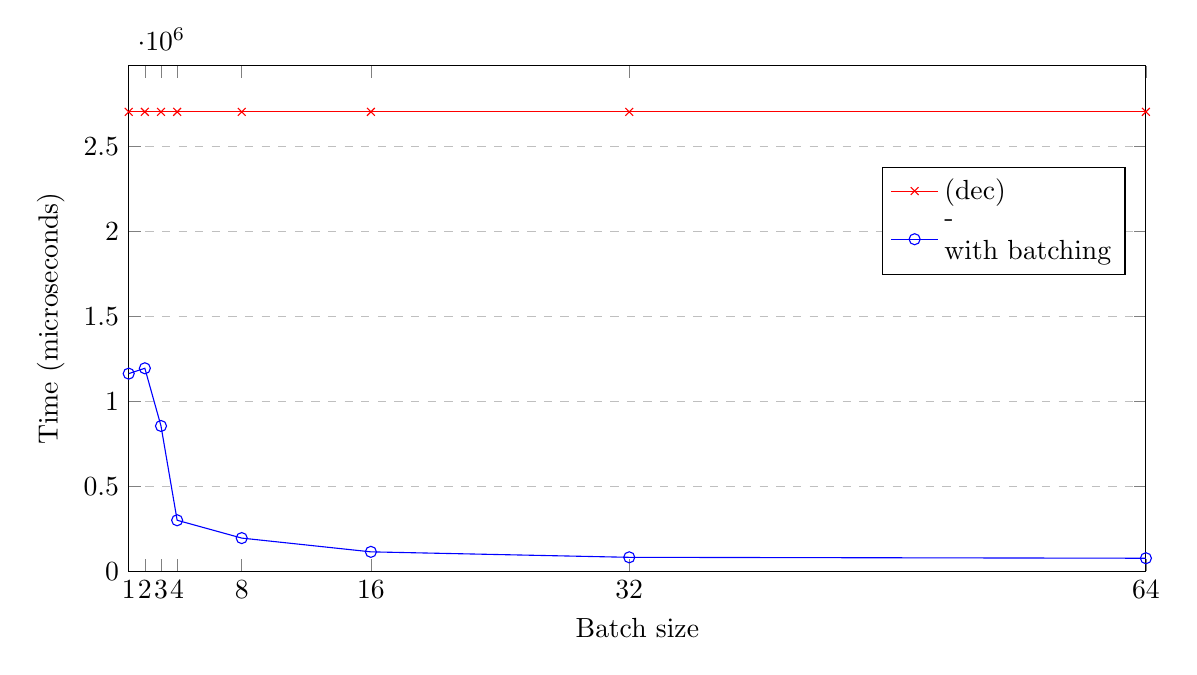
\begin{tikzpicture}
\begin{axis}[
    height=8cm,
    width=14.5cm,
    xlabel={Batch size},
    ylabel={Time (microseconds)},
    xmin=1, xmax=64,
    ymin=0,
    xtick={1,2,3,4,8,16,32,64},
    ymajorgrids=true,
    grid style=dashed,
    legend style={at={(0.98,0.8)}},
    legend style={cells={align=left}},
    legend cell align={left},
    legend entries = {\llinux (dec),\llinux-\memsc\\with batching}
]

\addplot[color=red, mark=x] coordinates {
  (1,\Cf)(2,\Cf)(3,\Cf)(4,\Cf)(8,\Cf)(16,\Cf)(32,\Cf)(64,\Cf)
};

\addplot[color=blue, mark=o] coordinates {
  (1,\Fa)(2,\Fb)(3,\Fc)(4,\Fd)(8,\Fe)(16,\Ff)(32, \Fg)(64, \Fh)
};

\end{axis}
\end{tikzpicture}
\caption{Comparison of batched system calls performance against standard
  \llinux for different batch sizes}
\label{fig:batched}
\end{figure}

\newcommand{\Ga}{\xintfloatexpr [-13] (\Fa-\Cf)*100/\Cf\relax}
\newcommand{\Gb}{\xintfloatexpr [-13] (\Fb-\Cf)*100/\Cf\relax}
\newcommand{\Gc}{\xintfloatexpr [-13] (\Fc-\Cf)*100/\Cf\relax}
\newcommand{\Gd}{\xintfloatexpr [-13] (\Fd-\Cf)*100/\Cf\relax}
\newcommand{\Ge}{\xintfloatexpr [-13] (\Fe-\Cf)*100/\Cf\relax}
\newcommand{\Gf}{\xintfloatexpr [-13] (\Ff-\Cf)*100/\Cf\relax}
\newcommand{\Gg}{\xintfloatexpr [-13] (\Fg-\Cf)*100/\Cf\relax}
\newcommand{\Gh}{\xintfloatexpr [-13] (\Fh-\Cf)*100/\Cf\relax}

Looking at these results the first thing we notice is that by executing the
system calls in batches of 2 might not result in performance improvement.
Instead, it might actually slightly worsen the execution time. This possibly
happens due to unfavorable scheduling combinations between the decoupled thread
and its \memsc worker.

However, with batches of 3 and 4 there is quite a large reduction of the
execution time. For batches of larger sizes, execution time continues to
decrease but the reduction is not as significant. Table
\ref{tab:batched_decrease} summarizes the percentage decrease in the execution
time of the benchmark when compared to standard \llinux. We notice that by
doing batches of 4 system calls there is already a reduction of almost 90\% of
the original execution time and the program actually even runs faster compared
to when running in non-decoupled mode (Table \ref{tab:block_single}). The time
reduction percentage can go up to 97.2\% for the maximum available batch size.

These results indicate that decoupled applications can significantly increase
their performance by doing system calls in small batches of 3 or 4. This is an
important observation since it is much easier for applications to prepare small
batches consisting of a few system calls as opposed to batches of tens of
system calls.

\begin{table}[h]
\centering
\scalebox{0.935}{
  \begin{tabular}{ |p{1.9cm}|p{1.22cm}|p{1.22cm}|p{1.22cm}|p{1.22cm}|p{1.22cm}|p{1.22cm}|p{1.22cm}|p{1.22cm}| }
 \hline
    Batch Size & 1 & 2 & 3 & 4 & 8 & 16 & 32 & 64 \\
 \hline
 \hline
    Exec Time & \Ga\% & \Gb\% & \Gc\% & \Gd\% & \Ge\% & \Gf\% & \Gg\% & \Gh\% \\
 \hline
\end{tabular}}
  \caption{Percentage decrease of execution time for different batch sizes over
  standard \llinux in decoupled mode}
\label{tab:batched_decrease}
\end{table}

This experiment was repeated with system calls other than getppid and the
results were found to be proportionally similar.

\subsection{System Throughput}

Next, the system call throughput of the system was evaluated. In this
experiment 2 applications (2 instances of the microbenchmark) ran decoupled in
parallel in the 1st and 2nd physical CPU correspondingly. The purpose of this
experiment was to see how many system calls per second the \llinux kernel can
handle with and without the \memsc patch.

To ensure that the applications started their execution roughly at the same
time, an intermediate shell script was used. This short script works by simply
sending a SIGSTOP signal to itself in order to transition to a sleep state.
When it wakes up, it uses the \emph{exec} command to load the benchmarking
program on its address space and execute it. After launching both applications
this way, the SIGCONT signal was sent to both of them with a single
\emph{killall} command in order to start their execution.

In order to measure the throughput, \llinux was modified and an atomic counter
for counting all system call requests from all system processes was added. A
new system call that returns the value of this counter was added as well. Using
this system call, the main benchmarking program was able to calculate the
system throughput by reading the atomic counter before and after executing the
getppid programs. The throughput was measured for different time intervals (5,
10, 20, and 30 seconds) and the results were found to be consistent.

The results collected are presented in Table \ref{tab:throughput_sync} and
Table \ref{tab:throughput_batch}. Additionally, Figure \ref{fig:throughput}
serves as a visual representation of these numbers. The system call throughput
was calculated for standard \llinux with and without decoupling, for
\llinux-\memsc with synchronous system calls, and for \llinux-\memsc with
asynchronous system calls and different batch sizes.

\newcommand\Hnodec{290341}
\newcommand\Hipi{37455}

\newcommand\Ha{133397}
\newcommand\Hb{136260}
\newcommand\Hc{197806}
\newcommand\Hd{485253}
\newcommand\He{603365}
\newcommand\Hf{1036953}
\newcommand\Hg{1600792}
\newcommand\Hh{2205457}

\begin{table}[h]
\centering
  \begin{tabular}{ |p{2.9cm}|p{0.7cm}|p{2cm}| }
 \hline
    OS kernel & dec & Throughput \\
 \hline
 \hline
    \llinux & no & \num{\Hnodec} \\
 \hline
    \llinux & yes & \num{\Hipi} \\
 \hline
    \llinux-\memsc & yes & \num{\Ha} \\
 \hline
\end{tabular}
  \caption{Throughput (system calls per second) per kernel and execution mode}
\label{tab:throughput_sync}
\end{table}

\begin{table}[h]
\centering
  \begin{tabular}{ |p{2cm}|p{1.3cm}|p{1.3cm}|p{1.3cm}|p{1.3cm}|p{1.6cm}|p{1.6cm}|p{1.6cm}| }
 \hline
    Batch Size & 2 & 3 & 4 & 8 & 16 & 32 & 64 \\
 \hline
 \hline
    Throughput & \num{\Hb} & \num{\Hc} & \num{\Hd} & \num{\He} & \num{\Hf} & \num{\Hg} & \num{\Hh} \\
 \hline
\end{tabular}
  \caption{Throughput (system calls per second) per batch size for
  \llinux-\memsc}
\label{tab:throughput_batch}
\end{table}

As with all previous experiments' results, we notice that \memsc with
decoupling performs better than standard \llinux with decoupling. Specifically,
the system call throughput is increased by
{\the\numexpr(\Ha-\Hipi)*100/\Hipi\relax}\% in this case.

\begin{figure}[h!]
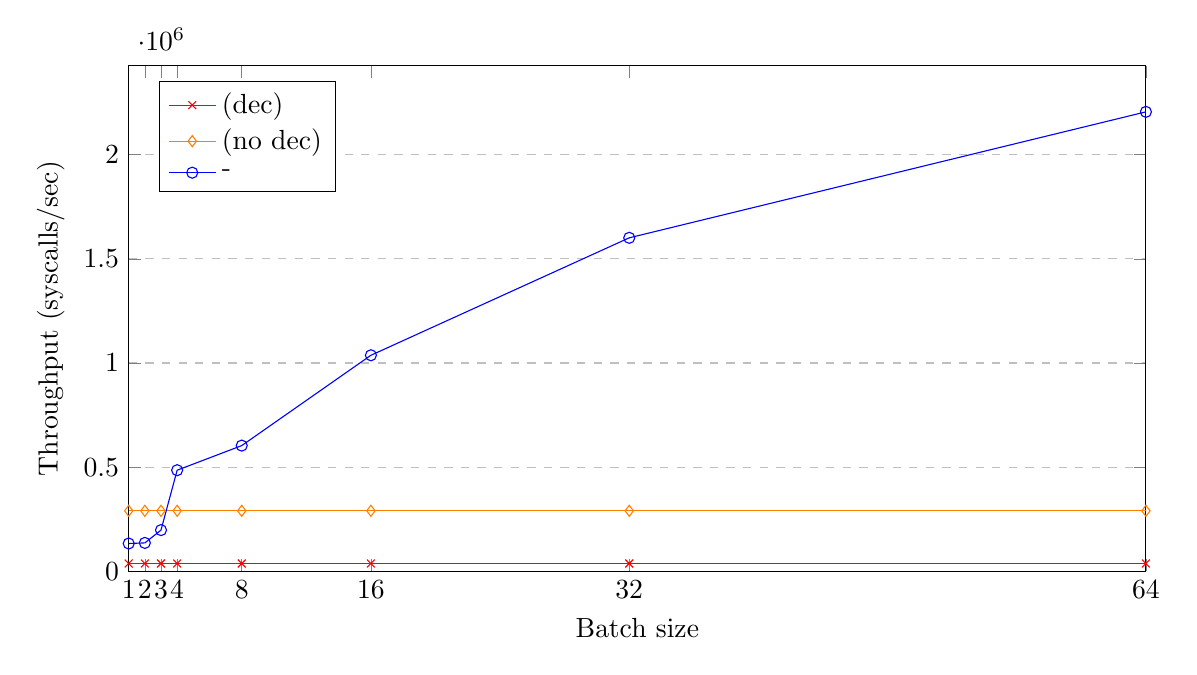
\begin{tikzpicture}
\begin{axis}[
    height=8cm,
    width=14.5cm,
    xlabel={Batch size},
    ylabel={Throughput (syscalls/sec)},
    xmin=1, xmax=64,
    ymin=0,
    xtick={1,2,3,4,8,16,32,64},
    ymajorgrids=true,
    grid style=dashed,
    legend pos=north west,
    legend cell align={left},
    legend entries = {\llinux (dec),\llinux (no dec),\llinux-\memsc}
]

\addplot[color=red, mark=x] coordinates {
  (1,\Hipi)(2,\Hipi)(3,\Hipi)(4,\Hipi)(8,\Hipi)(16,\Hipi)(32,\Hipi)(64,\Hipi)
};

\addplot[color=orange, mark=diamond] coordinates {
  (1,\Hnodec)(2,\Hnodec)(3,\Hnodec)(4,\Hnodec)(8,\Hnodec)(16,\Hnodec)(32,\Hnodec)(64,\Hnodec)
};

\addplot[color=blue, mark=o] coordinates {
  (1,\Ha)(2,\Hb)(3,\Hc)(4,\Hd)(8,\He)(16,\Hf)(32, \Hg)(64, \Hh)
};

\end{axis}
\end{tikzpicture}
\caption{Comparison of system call throughput between \llinux with and without
  decoupling and \llinux-\memsc for different batch sizes}
\label{fig:throughput}
\end{figure}

Additionally, from the \memsc results in batched mode, we notice that this time
batches of larger sizes have a bigger impact on performance. This is because
the processes are allowed to run for more time and the individual improvements
of each process are accumulated. For batches of 4, the system throughput is
already higher than when standard \llinux without decoupling is used. In
comparison to standard \llinux with decoupling, the throughput was increased by
{\the\numexpr(\Hd-\Hipi)*100/\Hipi\relax}\% for batches of 4 and by
{\the\numexpr(\Hh-\Hipi)*100/\Hipi\relax}\% for batches of 64.

This experiment was repeated for a larger number (4, 6, and 8) of decoupled
threads equally divided between the two cores. However due to the limited
physical resources, at any time only two out of these threads were able to
execute in parallel. The system throughput seemed to increase slightly with
more decoupled threads.

\section{General-Purpose Benchmarks Using Uclibc-Memsc}

The second part of the evaluation was done using the standard Unix dd and ls
programs. The busybox \cite{busybox} implementation of these utilities was
used, as it was included in the buildroot image. The whole busybox binary was
linked dynamically against uclibc-memsc, the modified C library, in order to
assess its execution using \memsc. No modification of the binary was required.

Since the root file system was not backed by a block device, all file
operations issued by these benchmarks were performed directly in memory.
Measuring execution time for these benchmarks was done using the time program.

\subsection{File Copying}

The dd program was used for copying files of different sizes and determining
whether file system operations are faster with \memsc. The program was called
with bs=512 which is the default value. The bs parameter of dd specifies the
number of bytes up to which dd reads and writes at a time. So one read and one
write system call were issued for copying each chunk of 512 bytes from the
original file to the new file.

The original file was created as a sparse file using the truncate command. Even
though the original sparse file occupied no storage, the dd command had to
allocate file system space (in this case memory) for the new file. The
benchmark was repeated for different file sizes. The maximum file size in this
benchmark was limited by the memory allocated to \llinux which was in turn
limited by the amount of physical system memory.

\break

\newcommand{\Ia}{1.43}
\newcommand{\Ib}{7.03}
\newcommand{\Ic}{14.02}
\newcommand{\Id}{20.87}
\newcommand{\Ie}{27.88}

\newcommand{\Ja}{0.83}
\newcommand{\Jb}{3.98}
\newcommand{\Jc}{7.95}
\newcommand{\Jd}{11.9}
\newcommand{\Je}{15.81}

\begin{figure}[h!]
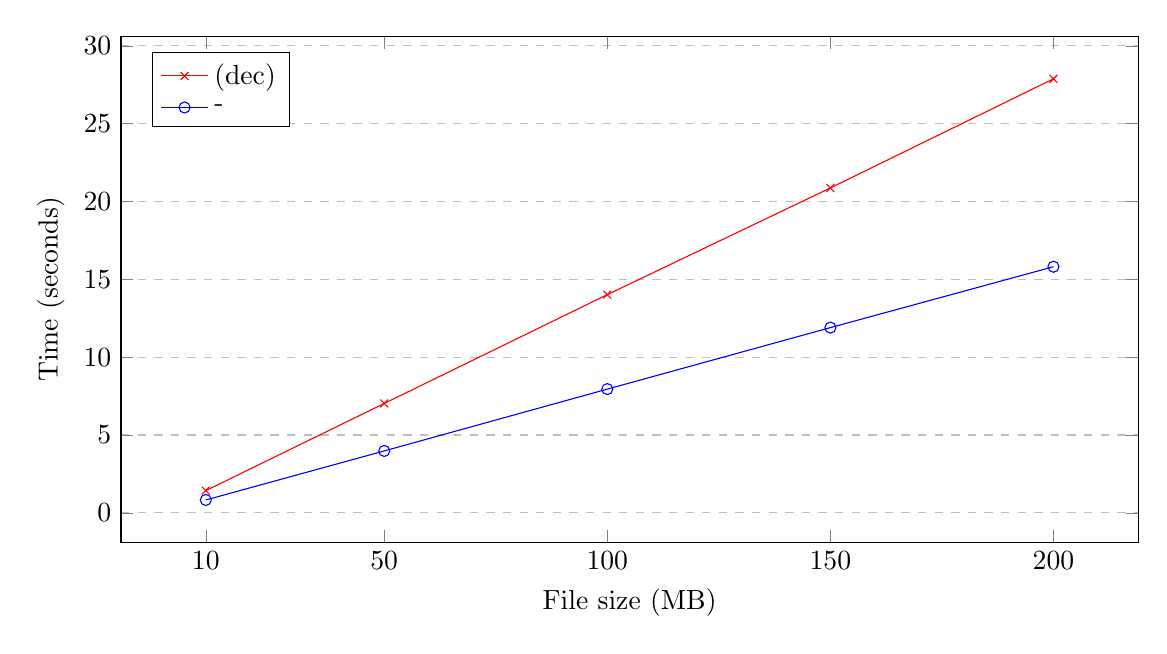
\begin{tikzpicture}
\begin{axis}[
    height=8cm,
    width=14.5cm,
    xlabel={File size (MB)},
    ylabel={Time (seconds)},
    xtick={10,50,100,150,200},
    ymajorgrids=true,
    grid style=dashed,
    legend pos=north west,
    legend cell align={left},
    legend entries = {\llinux (dec),\llinux-\memsc}
]

\addplot[color=red, mark=x] coordinates {
  (10,\Ia)(50,\Ib)(100,\Ic)(150,\Id)(200,\Ie)
};

\addplot[color=blue, mark=o] coordinates {
  (10,\Ja)(50,\Jb)(100,\Jc)(150,\Jd)(200,\Je)
};

\end{axis}
\end{tikzpicture}
\caption{Execution times for the dd benchmark with and without \memsc}
\label{fig:dd}
\end{figure}

% this doesn't work, pffffffff latex...
% \newcommand{\Ka}{\xintfloatexpr [-13] (\Ia-\Ja)*100/\Ja\relax}
% Percentages: \Ka . \Kb . \Kc . \Kd . \Ke

\newcommand{\Ka}{72.3}
\newcommand{\Kb}{76.6}
\newcommand{\Kc}{76.4}
\newcommand{\Kd}{75.4}
\newcommand{\Ke}{76.3}

\begin{figure}[h!]
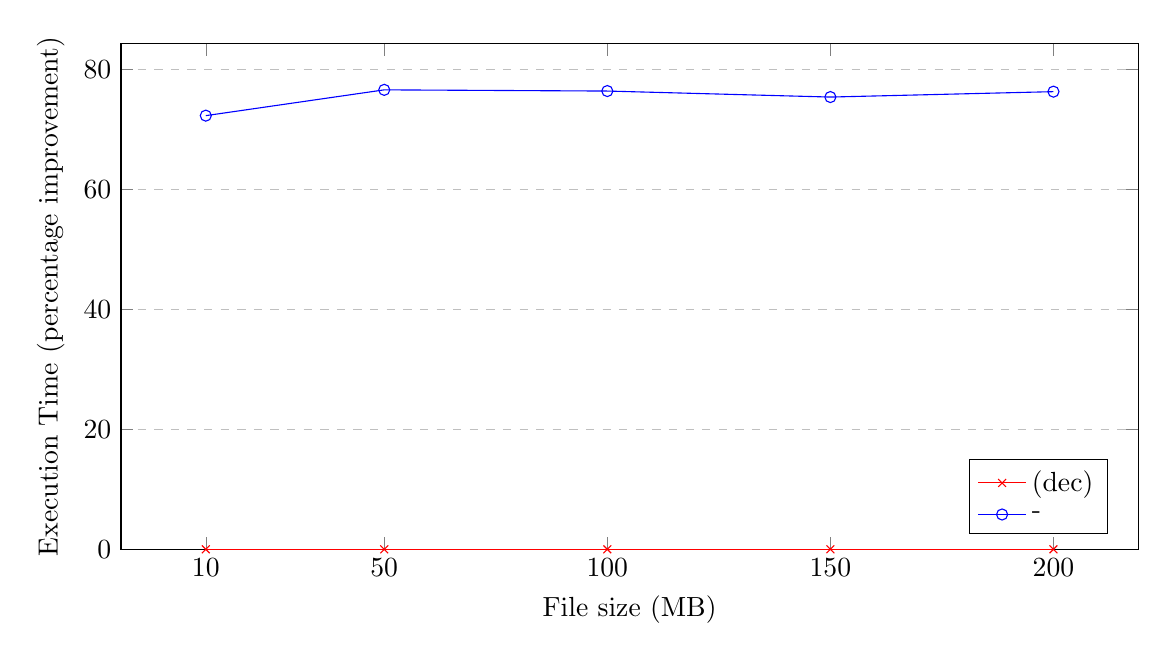
\begin{tikzpicture}
\begin{axis}[
    height=8cm,
    width=14.5cm,
    xlabel={File size (MB)},
    ylabel={Execution Time (percentage improvement)},
    ymin=0,
    xtick={10,50,100,150,200},
    ymajorgrids=true,
    grid style=dashed,
    legend pos=south east,
    legend cell align={left},
    legend entries = {\llinux (dec),\llinux-\memsc}
]

\addplot[color=red, mark=x] coordinates {
  (10,0)(50,0)(100,0)(150,0)(200,0)
};

\addplot[color=blue, mark=o] coordinates {
  (10,\Ka)(50,\Kb)(100,\Kc)(150,\Kd)(200,\Ke)
};

\end{axis}
\end{tikzpicture}
\caption{Execution time percentage improvement for the dd benchmark with
  \memsc compared to standard \llinux with decoupling}
\label{fig:dd_improvement}
\end{figure}

\break

It seems that even copying a sparse file in Linux populates its page cache with
zero-filled pages. This results in subsequent copies of the same file being
faster than the first one. For this reason, the original file was deleted and
created again between each test in order to ensure a cold page cache.

As shown in Figure \ref{fig:dd}, \memsc outperformed standard \llinux for all
file sizes. Figure \ref{fig:dd_improvement} shows the percentage improvement
over standard \llinux with decoupling. This remains pretty consistent
independently of the file size and is around 76\%.

\subsection{Directory Listing}

For the directory listing benchmark, ls was run in directories with different
amounts of files. The ls program was run with the -l option in order to force
it to issue a stat system call for each file listed. Its output was redirected
to a file in order to avoid any overheads related to the terminal emulator,
line buffering, and text rendering.

\newcommand{\La}{0.21}
\newcommand{\Lb}{0.9}
\newcommand{\Lc}{1.77}
\newcommand{\Ld}{2.64}

\newcommand{\Ma}{0.16}
\newcommand{\Mb}{0.64}
\newcommand{\Mc}{1.23}
\newcommand{\Md}{1.84}

\begin{figure}[h]
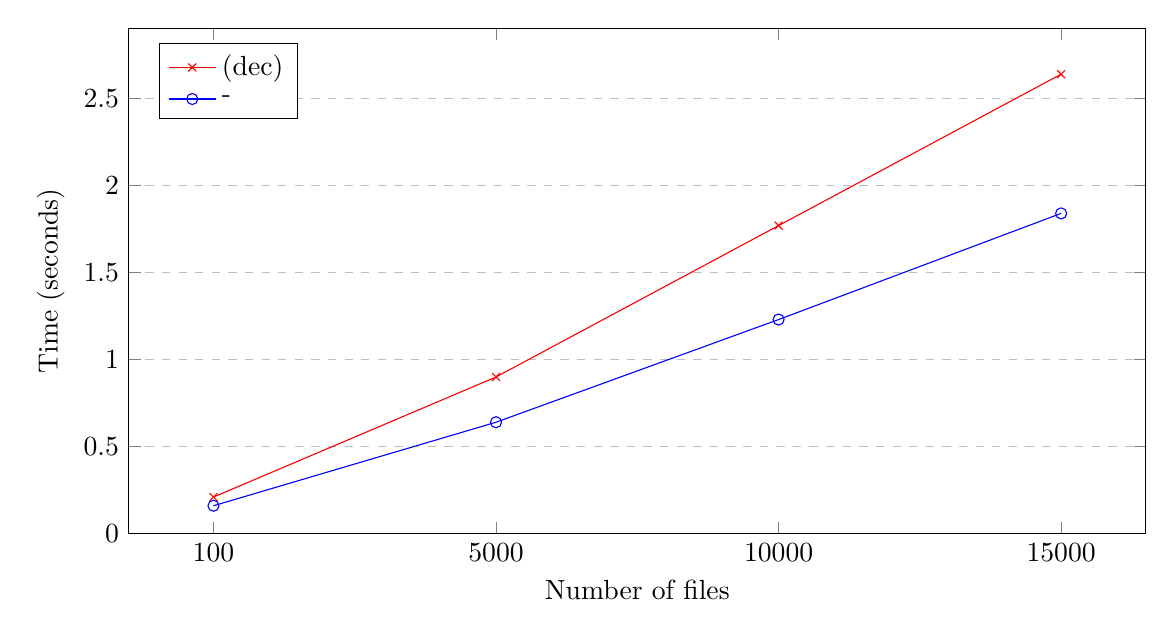
\begin{tikzpicture}
\begin{axis}[
    symbolic x coords={100,5000,10000,15000},
    height=8cm,
    width=14.5cm,
    xlabel={Number of files},
    ylabel={Time (seconds)},
    ymin=0,
    xtick={100, 5000, 10000, 15000},
    ymajorgrids=true,
    grid style=dashed,
    legend pos=north west,
    legend cell align={left},
    legend entries = {\llinux (dec),\llinux-\memsc}
]

\addplot[color=red, mark=x] coordinates {
  (100,\La)(5000,\Lb)(10000,\Lc)(15000,\Ld)
};

\addplot[color=blue, mark=o] coordinates {
  (100,\Ma)(5000,\Mb)(10000,\Mc)(15000,\Md)
};

\end{axis}
\end{tikzpicture}
\caption{Execution times for the ls -l benchmark with and without \memsc}
\label{fig:ls}
\end{figure}

The resulting execution times are presented in Figure \ref{fig:ls} as a graph.
Once again, \memsc performed better for all test cases with the benefits
increasing for a larger number of files. Figure \ref{fig:ls_improvement}
depicts execution time percentage improvements. \memsc shows an improvement of
31\% over standard \llinux for listing 100 files and an improvement of 43\% for
listing 15000 files.

\newcommand{\Na}{31.25}
\newcommand{\Nb}{40.62}
\newcommand{\Nc}{43.9}
\newcommand{\Nd}{43.47}

\begin{figure}[h]
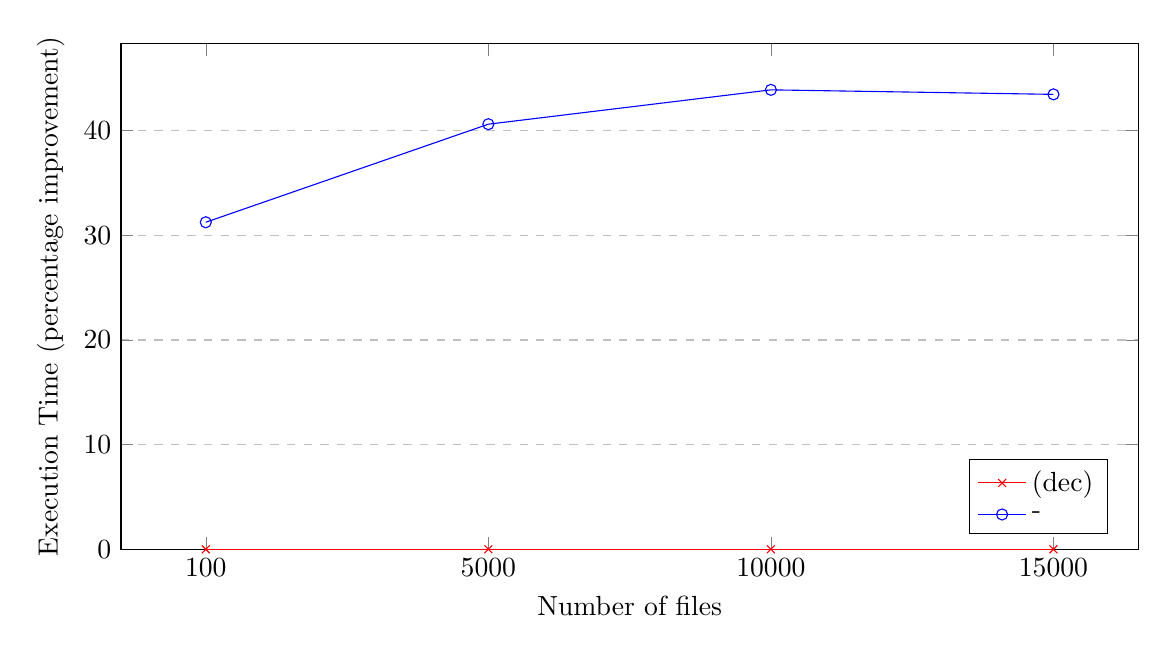
\begin{tikzpicture}
\begin{axis}[
    symbolic x coords={100,5000,10000,15000},
    height=8cm,
    width=14.5cm,
    xlabel={Number of files},
    ylabel={Execution Time (percentage improvement)},
    ymin=0,
    xtick={100, 5000, 10000, 15000},
    ymajorgrids=true,
    grid style=dashed,
    legend pos=south east,
    legend cell align={left},
    legend entries = {\llinux (dec),\llinux-\memsc}
]

\addplot[color=red, mark=x] coordinates {
  (100,0)(5000,0)(10000,0)(15000,0)
};

\addplot[color=blue, mark=o] coordinates {
  (100,\Na)(5000,\Nb)(10000,\Nc)(15000,\Nd)
};

\end{axis}
\end{tikzpicture}
\caption{Execution time percentage improvement for the ls -l benchmark with
  \memsc compared to standard \llinux with decoupling}
\label{fig:ls_improvement}
\end{figure}
